\chapter{Using light waves to measure small distance changes (Michelson interferometer)}

\section{Introduction}

With the basic properties of waves and wave interference established (via the ripple tank) and the same behavior
demonstrated in light (via the laser-based modern version of Young's double slit experiment) we are now finally ready to
look at a Michelson interferometer. This technology is the basis of the LIGO experiment. You may want to refer back to
the introduction of Lab~\ref{cha:ripple-tank} to remind yourself of some details. LIGO itself is a large experiment that has
been constructed over several decades of work and technology development, and so is many orders of magnitude more
precise and sensitive than what we can do in an hour on a lab bench. Nevertheless, the basic principles are the same.

%\section{Learning Goals}

\section{Team roles}

\begin{steps}
	\item \textbf{Decide on roles} for each group member.
\end{steps}

The available roles are:

\begin{itemize}
	\item Facilitator: ensures time and group focus are efficiently used
	\item Scribe: ensures work is recorded
	\item Technician: oversees apparatus assembly, usage
	\item Skeptic: ensures group is questioning itself
\end{itemize}

These roles can rotate each lab, and you will report at the end of the lab report on how it went for each role. If you have fewer than 4 people in your group, then some members will be holding more than one role. For example, you could have the skeptic double with another role. Consider taking on a role you are less comfortable with, to gain experience and more comfort in that role.

Additionally, if you are finding the lab roles more restrictive than helpful, you can decide to co-hold some or all roles, or think of them more like functions that every team needs to carry out, and then reflecting on how the team executed each function.

\section{Add members to Canvas lab report assignment group}

\begin{steps}
	\item On Canvas, navigate to the People section, then to the ``Lab 3 Groups'' tab. Find a group that is not yet used, and have each person in your group add themselves to that same lab group.
\end{steps}

This enables group grading of your lab report. Only one person will submit the group report, and all members of the group will receive the grade and have access to view the graded assignment.

\section{Observation experiment: demonstration of the interferometer}

\subsection{Goal}

Observe the flow of light in the Michelson interferometer simulation.

\subsection{Available equipment}

\begin{itemize}
	\item A virtual Michelson interferometer found at \url{https://www.geogebra.org/m/msfpudej}
	\begin{itemize}
		\item Note: in the sim, do not zoom in and out by scrolling --- when this happens, the coordinate system appears to shrink and expand, leading to the mirrors seeming to move in space.
	\end{itemize}
\end{itemize}

\subsection{Rubrics to be assessed for this section}

None.

\section{Steps}

\begin{steps}
	\item Load the virtual apparatus at the address listed in the available equipment section.
	
	\item Click the refresh button in the simulation, to the right of the Zeit slider. This fixes a bug where the green wave does not fully display.

	\item Slide Zeit (German for "time") to the left to equal 0. Uncheck "Weg Spiegel 1" (wave path 1)
\end{steps}

This is the Michelson interferometer, invented by Albert Michelson, a physicist whose family immigrated to the USA from Poland when he was 2 years old. He grew up in mining camps in California and Nevada and went on to found the physics department here at UChicago. Let's walk through the operation of the interferometer step by step. A schematic of the setup with parts labeled is found in Figure\ \ref{mir:fig:setup}.

\begin{figure}
	\centering
	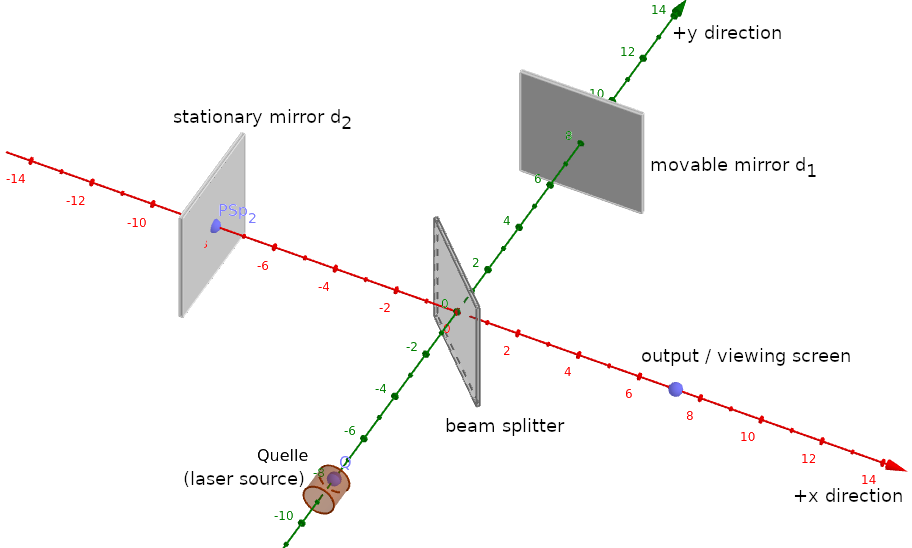
\includegraphics[width=\textwidth]{michelson-interferometer-remote/michelson-setup-geogebra}
	\caption{Diagram of the Michelson interferometer simulation with parts labeled.}\label{mir:fig:setup}
\end{figure}

\begin{steps}
	\item Select "Animation" and watch as the wave leaves the laser source and select it again to pause as the wave encounters the beam splitter.
\end{steps}

The beam splitter is a device that reflects some of the beam and transmits the rest. This one is a 50/50 beam splitter, so it splits the beam into equal parts.

\begin{steps}
	\item Select "Animation" again to watch the reflected part of the beam travel until it reaches the output/viewing screen. You'll watch the transmitted part of the beam at a later step. For now it is not displayed. \textit{If the reflected beam does not appear, refresh the animation using the circular arrow button to the right of the Zeit slider.}
\end{steps}

This reflected beam travels to the stationary mirror a distance $d_2$, reflects from that mirror, travels directly through the beam splitter on the way back, and exits the device to be seen on the viewing screen. (we ignore the part that is reflected when it strikes the beam splitter on the way back). The arrow that appears at the output represents the phase of the wave that is passing that point. For example, when the wave is cresting, the arrow points up, and when the wave is at a trough, the arrow points down.

\begin{steps}
	\item Move Zeit back to zero. Check the box for Weg Spiegel 1 and uncheck Weg Spiegel 2. Watch the animation again to follow the path of the beam that is initially transmitted through the beam splitter.
\end{steps}

This beam strikes the mirror at $d_1$, which is movable using the slider on the left or by typing in the desired distance. The typing field accepts numbers with precision up to 4 decimal places.

\begin{steps}
	\item Move Zeit back to zero, check both boxes, and watch the beams overlap with each other at the output.
\end{steps}

In this way the original beam of light splits, and portions of the resulting beams are brought back together to interfere with each other. The black arrow represents the sum of the two waves. The direction is the phase and the length is proportional to the amplitude of the resulting wave.

\section{Testing experiment: testing the theory of wave interference}

\subsection{Goal}

Test if the theory of wave interference and path length difference predicts the correct behavior in the situation of the Michelson interferometer. This theory states that for two different sources of waves that are of the same, single wavelength, and which started out in phase, then constructive interference occurs at a location when the difference in travel distances (path lengths) between the two sources is an integer number of wavelengths. Destructive interference occurs when the path length difference is a half-integer, for example 0.5, 1.5, or 2.5 wavelengths.

\subsection{Available equipment}

\begin{itemize}
	\item A virtual Michelson interferometer as in the previous experiment.
\end{itemize}

\subsection{Rubrics to be assessed for this section}

\begin{itemize}
	\item \textbf{C4:} Is able to make a reasonable prediction based on a hypothesis
	\item \textbf{C7:} Is able to decide whether the prediction and the outcome agree/disagree
	\item \textbf{F1:} Is able to communicate the details of an experimental procedure clearly and completely
	\item \textbf{F2:} Is able to communicate the point of the experiment clearly and completely
\end{itemize}
See Appendix~\ref{cha:rubrics} for details.

\subsection{Suggestions for your experiment}

\begin{itemize}
	\item Ensure that all group members are familiar with how path length difference results in constructive and destructive interference.
	
	\item Examine the geometry of the setup to determine the path length of the beam that travels through each arm of the interferometer.
	
	\item Develop a specific prediction of what setting combinations of wavelength and mirror distance will result in different observable interference effects.
	
	\item Note that in the simulation, you can type in a mirror distance $d_1$ with a precision of 4 decimal places. Press enter after typing it in to save it and have the result displayed.
\end{itemize}

\subsection{Items to include in your report}

Relevant rubric rows from Appendix~\ref{cha:rubrics} are listed in parentheses.

\begin{enumerate}
	\item Clear statement of the hypothesis you are testing (C1, not assessed)
	\item Prediction that follows from the hypothesis, along with justification (C4)
	\item Description of experimental procedure to produce outcome (F1)
	\item Determination of how much the prediction agrees with the outcome (C7)
	\item A discussion of the findings of the experiment and why it's helpful (for you and/or for science) (F2)
\end{enumerate}

\section{Application experiment: measuring length changes with the interferometer}

\subsection{Goal}

The Michelson interferometer is used for LIGO since gravitational waves create very small vibrations in spacetime as they pass. These vibrations literally alter the distance between the beam splitter and mirror along one axis. This MI simulates this with a movable mirror. Using this virtual MI, \textbf{develop a procedure} to determine the change in mirror distance $d_1$ if given the image of the black arrow as displayed on the screen (the arrow's length is proportional to the brightness at that location and moment). \textbf{Demonstrate this procedure} with an example initial and final mirror position.

\textbf{Determine how small} a change in the mirror distance you can measure using your procedure (the \textit{resolution} of the instrument. \textbf{Identify methods} to improve this resolution. 

\subsection{Available equipment}

\begin{itemize}
	\item A virtual Michelson interferometer as in the previous experiment.
\end{itemize}

\subsection{Rubrics to be assessed for this section}

\begin{itemize}
	\item \textbf{D2:} Is able to design a reliable experiment that solves the problem
	\item \textbf{G2:} Is able to evaluate specifically how identified experimental uncertainties affect the data
	\item \textbf{G3:} Is able to describe how to minimize experimental uncertainty and actually do it
	\item \textbf{F1:} Is able to communicate the details of an experimental procedure clearly and completely
	\item \textbf{F2:} Is able to communicate the point of the experiment clearly and completely
\end{itemize}

See Appendix~\ref{cha:rubrics} for details.

\subsection{Suggestions for your experiment}

\begin{itemize}
	\item Remember that the laser wavelength $\lambda$ and the mirror distances are given in micrometers ($\mu$m). This makes it an infrared laser.
	
	\item Decide how you will measure the black arrow's length. This can many methods, for example holding up a ruler to the screen or taking a screenshot and measuring the pixel length in an image analysis program like ImageJ.
	
	\item Note that in the simulation, you can type in a mirror distance $d_1$ with a precision of 4 decimal places. Press enter after typing it in to save it and have the result displayed.
\end{itemize}

\subsection{Items to include in your report}

Relevant rubric rows from Appendix~\ref{cha:rubrics} are listed in parentheses.

\begin{enumerate}
	\item Description of procedure to use image of black arrow to determine the change in mirror distance $d_1$ (D2, F1)
	\item Demonstration of this procedure
	\item Determination of measurement resolution (G2)
	\item Identification of ways to improve this resolution (G3)
	\item A discussion of the findings of the experiment and why it's helpful (for you and/or for science) (F2)
\end{enumerate}

\section{Group functioning}

\begin{steps}
	\item A 100--200 word reflection on group dynamics. Address the following topics: who did what in the lab, how did you work together, how group roles functioned, what successes and challenges in group functioning did you have, and what do you want to continue doing or do differently?
\end{steps}

\section{Individual homework}

\begin{enumerate}
	\item If you were to add a mirror between the beam splitter and the movable mirror, such that the light struck the movable mirror, then our new mirror, then back to the movable mirror, then back to the beam splitter, how would this change the resolution of your measuring device from the application experiment, if at all?
	
	\item Given the resolution of your instrument that you found in the application experiment, what are examples of objects at that length scale that you would be able to use this to measure with 1\% accuracy? You can use this website as a starting point: \url{https://htwins.net/scale2/}
\end{enumerate}